% !TEX program = lualatex
\documentclass[12pt,a4paper]{article}
\usepackage{graphicx}
\usepackage{fontspec}
\setmonofont{Latin Modern Mono}
\usepackage{xcolor}
\usepackage{listings}
\usepackage{geometry}
\usepackage{fancyhdr}
\usepackage{hyperref}
\usepackage{booktabs} 
\usepackage{float}    
\usepackage{amsmath}

% =======================================================
%  USER CONFIGURATION
% =======================================================
\newcommand{\labNo}{Lab 11}
\newcommand{\labTopic}{PL/pgSQL Named Blocks: Functions and Procedures}
\newcommand{\courseCode}{CSE 4308}
\newcommand{\courseTitleShort}{DBMS Lab}
\newcommand{\courseTitleLong}{DATABASE MANAGEMENT SYSTEMS LAB}
\newcommand{\instructorName}{Samnun Azfar, Jr. Lecturer, CSE\\ Samia Nawsheen, Jr. Lecturer, CSE}
\newcommand{\academicYear}{AY25-26}

% --- SOLUTION TOGGLE ---
% Change \showsolutionstrue to \showsolutionsfalse to generate 
% the student version (hidden answers).
\newif\ifshowsolutions
 % \showsolutionstrue 
\showsolutionsfalse
% =======================================================

\geometry{margin=1in}

% -
% Header and Footer Configuration
% -
\pagestyle{fancy}
\fancyhf{}
\lhead{\labNo}                        % Uses variable
\rhead{\courseCode: \courseTitleShort} % Uses variables

% Centered footer with page number
\cfoot{\thepage}
% Ensure header/footer width matches text block
\setlength{\headwidth}{\textwidth}

% -
% Code Listing Style
% -
\definecolor{codegreen}{rgb}{0,0.6,0}
\definecolor{codegray}{rgb}{0.5,0.5,0.5}
\definecolor{codepurple}{rgb}{0.58,0,0.82}
\definecolor{backcolour}{rgb}{0.95,0.95,0.92}

\lstdefinestyle{mystyle}{
    backgroundcolor=\color{backcolour},
    commentstyle=\color{codegreen},
    keywordstyle=\color{magenta},
    numberstyle=\tiny\color{codegray},
    stringstyle=\color{codepurple},
    basicstyle=\ttfamily\footnotesize,
    breaklines=true,
    captionpos=b,
    keepspaces=true,
    numbers=left,
    numbersep=5pt,
    tabsize=2,
    frame=single,
    numbers=none,
    columns=fullflexible,
    showspaces=false,
    showstringspaces=false,
    showtabs=false,
}

\lstset{style=mystyle}

% Images: found next to this file (local compile_labs.sh) or via the
% lab folder when compiled from the project root (Overleaf).
\graphicspath{{lab_11_function_procedure/}}

\begin{document}

% --
% TITLE PAGE
% --
\begin{titlepage}
    \centering
    \vspace*{2\baselineskip}

    \rule{14cm}{2pt}\vspace*{-0.8\baselineskip}\vspace*{1.5pt}
    \rule{14cm}{0.5pt}\vspace{2\baselineskip}

    {\Huge\bfseries\scshape \labNo\par} % Uses variable
    \vspace{3mm}
    {\Large \labTopic} % Uses variable
    \vspace{3mm}

    \rule{14cm}{0.5pt}\vspace*{-0.7\baselineskip}\vspace{2.5pt}
    \rule{14cm}{2pt}

    \vspace{2\baselineskip}

    {\Large\bfseries \courseCode\par} % Uses variable
    \vspace{1\baselineskip}
    {\large \courseTitleLong\par} % Uses variable

    \vfill
    {\normalsize Prepared by:\\ \instructorName\par} % Uses variable
    {\normalsize Academic Year: \academicYear\par} % Uses variable
\end{titlepage}

\newpage
\tableofcontents
\newpage

% =======================================================
% SECTION: LAB WORKFLOW
% =======================================================
\section{Lab Workflow}



\textit{Repeat this subsection for every single lab.}

\begin{enumerate}
\item Connect to the internet by running nmtui in terminal, add a dsl connection, then go back and activate that dsl connection. Make sure that your net id is not being used in any other pc or router, if you face any issue, use any other net id from your friends which is not being used.

\item Download all the files posted in the google classroom.

\item Disconnect from the \textbf{dsl} connection via nmtui, connect to the ethernet/wired connection via nmtui. If no such connection exists, create an \textbf{ethernet} connection  and then activate.

    \item \textbf{Create Your Role and Database}

Inside the PostgreSQL shell, create your own role (user) and database.

1. In the Linux terminal:
\begin{lstlisting}[language=bash]
psql
\end{lstlisting}

Expected prompt:
\begin{lstlisting}
cse=#
\end{lstlisting}

2. Create Your Role and Database

Copy and run the following commands inside PostgreSQL:
\begin{lstlisting}[language=SQL]
-- 1. Terminate existing database connections
SELECT pg_terminate_backend(pid)
FROM pg_stat_activity
WHERE datname = 'cse4308_12345'
  AND pid <> pg_backend_pid();

-- 2. Remove existing database
DROP DATABASE IF EXISTS cse4308_12345;

-- 3. Remove existing role
DROP ROLE IF EXISTS student_12345;

-- 4. Create role
CREATE ROLE student_12345 LOGIN;

-- 5. Set password
ALTER ROLE student_12345
WITH PASSWORD 'student12345';

-- 6. Create database
CREATE DATABASE cse4308_12345
OWNER student_12345;

-- 7. Grant privileges
GRANT ALL PRIVILEGES
ON DATABASE cse4308_12345
TO student_12345;
\end{lstlisting}

3. Exit PostgreSQL:

   \begin{lstlisting}[language=SQL]
   \q
   \end{lstlisting}

\item \textbf{Connect Using Your Newly Created User}

1. Connect to Your Database:

   Use the following command to log in as the \texttt{student\_12345} user:

   \begin{lstlisting}[language=SQL]
   psql -h localhost -U student_12345 -d cse4308_12345
   \end{lstlisting}

2. Verify the Connection:

   Verify that you are connected to the correct database with the following command:

   \begin{lstlisting}[language=SQL]
   \conninfo
   \end{lstlisting}

   Expected output:

   \begin{lstlisting}
   Database: cse4308_12345, User: student_12345
   \end{lstlisting}

3. Exit PostgreSQL:

   \begin{lstlisting}[language=SQL]
   \q
   \end{lstlisting}

\item \textbf{Load the Lab SQL File (MUST be run outside psql)}

Load the SQL file that sets up the tables and inserts initial data.

1. Load the SQL File:

   Run the following command to load the lab SQL file:

   \begin{lstlisting}[language=SQL]
   psql -h localhost -U student_12345 -d cse4308_12345 -f /home/cse/Downloads/lab_11_setup.sql
   \end{lstlisting}

   This will:
   - Drop old tables (if they exist).
   - Create new tables.
   - Insert initial rows of data.

\item \textbf{Reconnect and Verify Tables}

After loading the SQL file, reconnect to PostgreSQL to verify that the tables have been created.

1. Reconnect to Your Database:

   \begin{lstlisting}[language=SQL]
   psql -h localhost -U student_12345 -d cse4308_12345
   \end{lstlisting}

2. Check Tables:

   Verify the tables have been created by listing them:

   \begin{lstlisting}[language=SQL]
   \dt
   \end{lstlisting}

3. View Table Data:

   Verify the data by running the following SQL queries:

   \begin{lstlisting}[language=SQL]
   SELECT * FROM <table_name>;
   \end{lstlisting}

\item Open a text editor and save it in the appropriate submission name format \\ \texttt{fullid\_CSE4308\_L11\_T1.sql}. You will use this text editor to write your solutions, make sure to save it after writing each solution. The structure of this file will be:
\begin{lstlisting}[language=SQL]
-- Task 1
INSERT INTO students (student_id, name, major, gpa)
VALUES (104, 'David', 'ME', 3.60);
--Task 2
SELECT name, gpa FROM students WHERE major = 'CSE';
\end{lstlisting}
\end{enumerate}
% =======================================================
% SECTION: DATABASE SCHEMA
% =======================================================
\newpage
\section{Database Schema \& Data Generation}
\textbf{Instructions:} Save this code as \texttt{lab\_11\_setup.sql} and run it using \texttt{\textbackslash i lab\_11\_setup.sql} in your \texttt{psql} terminal. This script generates a  e-commerce schema.

\begin{lstlisting}[language=SQL, caption={lab\_11\_setup.sql}]
-- 1. CLEANUP
DROP TABLE IF EXISTS order_items CASCADE;
DROP TABLE IF EXISTS orders CASCADE;
DROP TABLE IF EXISTS restock_logs CASCADE;
DROP TABLE IF EXISTS products CASCADE;
DROP TABLE IF EXISTS customers CASCADE;

-- 2. CREATE TABLES
CREATE TABLE customers (
    customer_id SERIAL PRIMARY KEY,
    name VARCHAR(100),
    region VARCHAR(50),
    loyalty_tier VARCHAR(20) -- 'Bronze', 'Silver', 'Gold', 'Platinum'
);

CREATE TABLE products (
    product_id SERIAL PRIMARY KEY,
    name VARCHAR(100),
    category VARCHAR(50),
    base_price NUMERIC(10, 2),
    stock_quantity INT
);

CREATE TABLE orders (
    order_id SERIAL PRIMARY KEY,
    customer_id INT REFERENCES customers(customer_id),
    order_date DATE,
    status VARCHAR(20), -- 'PENDING', 'PROCESSED', 'PARTIAL', 'BACKORDERED'
    total_value NUMERIC(12, 2) DEFAULT 0.00
);

CREATE TABLE order_items (
    item_id SERIAL PRIMARY KEY,
    order_id INT REFERENCES orders(order_id) ON DELETE CASCADE,
    product_id INT REFERENCES products(product_id),
    quantity INT,
    unit_price NUMERIC(10, 2)
);

CREATE TABLE restock_logs (
    log_id SERIAL PRIMARY KEY,
    product_id INT REFERENCES products(product_id),
    restock_date DATE,
    added_quantity INT
);

-- 3. DATA GENERATION
-- Insert 1000 Customers
INSERT INTO customers (name, region, loyalty_tier)
SELECT 
    'Customer_' || id,
    (ARRAY['North', 'South', 'East', 'West'])[floor(random() * 4 + 1)],
    (ARRAY['Bronze', 'Silver', 'Gold', 'Platinum'])[floor(random() * 4 + 1)]
FROM generate_series(1, 1000) AS id;

-- Insert 200 Products
INSERT INTO products (name, category, base_price, stock_quantity)
SELECT 
    'Product_' || id,
    (ARRAY['Electronics', 'Clothing', 'Groceries', 'Tools', 'Books'])[floor(random() * 5 + 1)],
    ROUND((random() * 500 + 10)::numeric, 2),
    floor(random() * 100 + 10)::INT
FROM generate_series(1, 200) AS id;

-- Insert 3000 Orders (All marked as PENDING initially)
INSERT INTO orders (customer_id, order_date, status)
SELECT 
    floor(random() * 1000 + 1)::INT,
    '2026-01-01'::DATE - (floor(random() * 365)::INT),
    'PENDING'
FROM generate_series(1, 3000);

-- Insert 9000 Order Items (Averaging 3 items per order)
INSERT INTO order_items (order_id, product_id, quantity, unit_price)
SELECT 
    floor(random() * 3000 + 1)::INT,
    floor(random() * 200 + 1)::INT,
    floor(random() * 5 + 1)::INT,
    0.00 -- To be updated based on product base price
FROM generate_series(1, 9000) ON CONFLICT DO NOTHING;

-- Fix the unit_price in order_items based on products table
UPDATE order_items oi
SET unit_price = p.base_price
FROM products p
WHERE oi.product_id = p.product_id;

-- Initial aggregation to set order total_values
UPDATE orders o
SET total_value = sub.total
FROM (
    SELECT order_id, SUM(quantity * unit_price) as total 
    FROM order_items 
    GROUP BY order_id
) sub
WHERE o.order_id = sub.order_id;
\end{lstlisting}
\begin{figure}
    \centering
    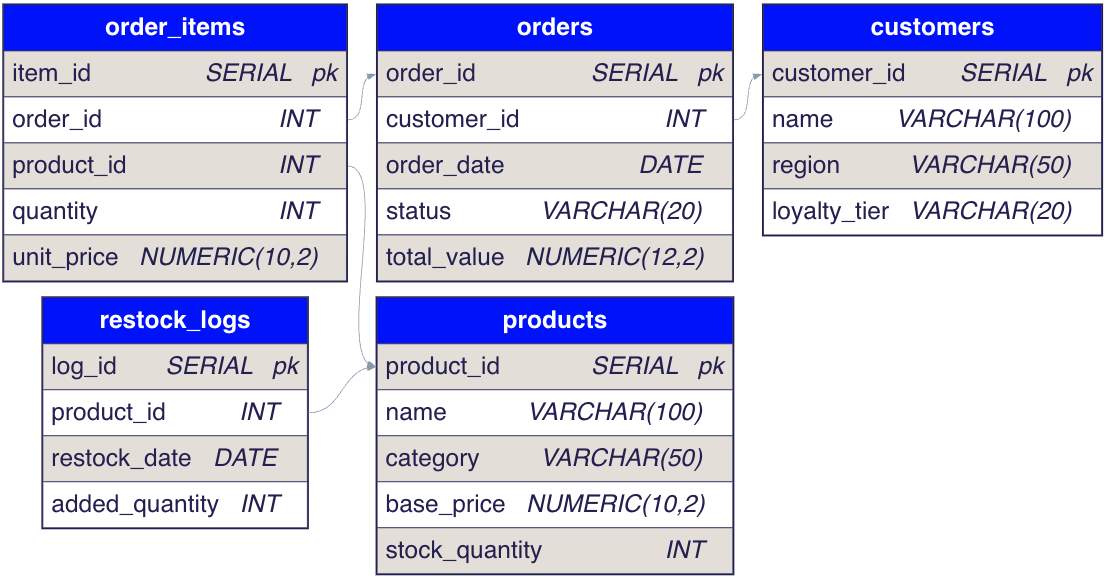
\includegraphics[width=0.7\linewidth]{lab_11_figure.png}
\end{figure}
% =======================================================
% SECTION: INTRODUCTION TO PL/pgSQL
% =======================================================
\newpage
\section{Introduction to Named Blocks}
Anonymous blocks (\texttt{DO \$\$}) evaluate procedural logic for single execution but are not persistently stored in the database schema. Persistent named blocks, referred to as subprograms, encapsulate procedural logic for reuse. In PostgreSQL, subprograms are classified into two primary constructs: \textbf{User-Defined Functions} and \textbf{Stored Procedures}.

% =======================================================
% SECTION: USER-DEFINED FUNCTIONS
% =======================================================
\section{User-Defined Functions}

A User-Defined Function is a named PL/pgSQL block that evaluates to a specific return type. Functions are invoked within expressions (e.g., a Data Manipulation Language \texttt{SELECT} statement) and structurally require a \texttt{RETURN} or \texttt{RETURN QUERY} statement. A defining characteristic of a function is that it executes entirely within the transaction scope of the invoking query; it cannot execute Transaction Control Language (TCL) commands such as \texttt{COMMIT} or \texttt{ROLLBACK}.

\subsection{Scalar and Table-Valued Functions}
A scalar function evaluates to a single, atomic value per invocation, utilizing the \texttt{RETURNS <datatype>} clause. Conversely, a table-valued function evaluates to a relational dataset, utilizing the \texttt{RETURNS TABLE} clause and the \texttt{RETURN QUERY} statement to populate the output relation.

\begin{lstlisting}[language=SQL, caption={Scalar Function Definition}]
	CREATE OR REPLACE FUNCTION calculate_customer_lifetime_value(p_cust_id INT)
	RETURNS NUMERIC AS $$
	DECLARE
	v_total_spent NUMERIC;
	BEGIN
	SELECT COALESCE(SUM(total_value), 0) INTO v_total_spent
	FROM orders
	WHERE customer_id = p_cust_id;
	
	RETURN v_total_spent;
	END;
	$$ LANGUAGE plpgsql;
\end{lstlisting}

% =======================================================
% SECTION: STORED PROCEDURES
% =======================================================
\section{Stored Procedures}



A Stored Procedure is a named PL/pgSQL block invoked via the \texttt{CALL} statement. Unlike functions, procedures do not evaluate to a direct return value (omitting the \texttt{RETURNS} clause) and are capable of autonomous transaction control. Procedures can initiate and terminate transactions using TCL commands (\texttt{COMMIT} and \texttt{ROLLBACK}). This capability dictates their use for bulk data manipulation, schema migrations, and batch processing workflows.

\begin{lstlisting}[language=SQL, caption={Stored Procedure with Transaction Control}]
	CREATE OR REPLACE PROCEDURE process_product_restock(
	p_product_id INT,
	p_added_qty INT
	)
	LANGUAGE plpgsql AS $$
	BEGIN
	UPDATE products
	SET stock_quantity = stock_quantity + p_added_qty
	WHERE product_id = p_product_id;
	
	IF NOT FOUND THEN
	RAISE EXCEPTION 'Product Identifier % does not exist.', p_product_id;
	END IF;
	
    INSERT INTO restock_logs (product_id, restock_date, added_quantity)
    VALUES (p_product_id, CURRENT_DATE, p_added_qty);

	-- Explicit Transaction Control
	COMMIT;
	END;
	$$;
\end{lstlisting}

% =======================================================
% SECTION: PARAMETER MODES
% =======================================================
\newpage
\section{Parameter Modes and Default Behavior}

Formal parameters in PL/pgSQL are assigned a mode that dictates the direction of data binding between the calling environment and the subprogram. The supported modes are \texttt{IN}, \texttt{OUT}, and \texttt{INOUT}.

\subsection{Implicit Default Behavior}
If a parameter mode is omitted during the formal parameter declaration, the PL/pgSQL compiler implicitly assigns the \texttt{IN} mode by default. Consequently, any unannotated parameter is strictly evaluated as a read-only constant within the subprogram's execution scope; attempting to mutate its state will trigger a compilation error.

\subsection{Mode Definitions}
\begin{itemize}
	\item \textbf{\texttt{IN} Mode:} Specifies that the formal parameter accepts an actual argument from the caller. It is lexically immutable within the subprogram body.
	\item \textbf{\texttt{OUT} Mode:} Specifies an uninitialized variable bound to the caller's environment. The subprogram assigns a value to it, which is transmitted back upon termination. When \texttt{OUT} parameters are present in a function, the \texttt{RETURNS} clause is typically omitted as the function implicitly returns a record of the \texttt{OUT} variables.
	\item \textbf{\texttt{INOUT} Mode:} A hybrid parameter that accepts an initialized actual argument from the caller, permits state mutation within the subprogram body, and transmits the modified state back to the caller upon termination.
\end{itemize}

% =======================================================
% SECTION: COMPREHENSIVE EXAMPLES
% =======================================================
\section{Integration of Parameter Modes}

The following examples demonstrate the simultaneous application of \texttt{IN}, \texttt{OUT}, and \texttt{INOUT} modes within a single subprogram.

\subsection{Function Implementation with Mixed Modes}
When a function incorporates \texttt{OUT} and \texttt{INOUT} parameters, it evaluates to a composite \texttt{RECORD} type containing the mutated variables.

\begin{lstlisting}[language=SQL, caption={Function integrating IN, OUT, and INOUT modes}]
	CREATE OR REPLACE FUNCTION evaluate_customer_loyalty(
	p_cust_id IN INT, -- Implicit or explicit IN: Read-only
	p_points_accrued INOUT NUMERIC,   -- Mutated and returned
	p_eligible_for_upgrade OUT BOOLEAN -- Calculated and returned
	)
	LANGUAGE plpgsql AS $$
	DECLARE
	v_current_tier VARCHAR;
	BEGIN
	-- Read the IN parameter
	SELECT loyalty_tier INTO v_current_tier
	FROM customers
	WHERE customer_id = p_cust_id;
	
	-- Mutate the INOUT parameter based on internal logic
	IF v_current_tier = 'Bronze' AND p_points_accrued < 5000.00 THEN
	p_points_accrued := p_points_accrued * 1.10; -- 10 percent point bonus
	END IF;
	
	-- Assign the OUT parameter
	IF p_points_accrued >= 2000.00 THEN
	p_eligible_for_upgrade := TRUE;
	ELSE
	p_eligible_for_upgrade := FALSE;
	END IF;
	
	-- No RETURN statement required; OUT/INOUT parameters form the implicit return record
	END;
	$$;
\end{lstlisting}

\textbf{Invocation:}
\begin{lstlisting}[language=SQL]
	-- The caller provides arguments only for IN and INOUT parameters.
	SELECT * FROM evaluate_customer_loyalty(1, 1500.00);
\end{lstlisting}

\subsection{Procedure Implementation with Mixed Modes}
Procedures utilizing mixed parameter modes are invoked via the \texttt{CALL} statement. The caller must provide initialized variables for \texttt{INOUT} parameters and target variables for \texttt{OUT} parameters to capture the modified states.

\begin{lstlisting}[language=SQL, caption={Procedure integrating IN, OUT, and INOUT modes}]
	CREATE OR REPLACE PROCEDURE process_category_discount(
	p_category IN VARCHAR,-- Read-only constraint
	p_discount_budget INOUT NUMERIC,   -- Mutated and returned to caller
	p_budget_status OUT VARCHAR -- Assigned and returned to caller
	)
	LANGUAGE plpgsql AS $$
	DECLARE
	v_product_count INT;
	BEGIN
	-- Utilize IN parameter for scalar subquery
	SELECT COUNT(*) INTO v_product_count
	FROM products
	WHERE category = p_category;
	
	-- Transform the INOUT parameter
	p_discount_budget := p_discount_budget - (v_product_count * 50.00);
	
	-- Initialize the OUT parameter
	IF p_discount_budget > 0 THEN
	p_budget_status := 'BUDGET_SURPLUS';
	ELSE
	p_budget_status := 'BUDGET_DEFICIT';
	END IF;
	
	-- Procedural Transaction Control
	COMMIT;
	END;
	$$;
\end{lstlisting}

\textbf{Invocation:}
\begin{lstlisting}[language=SQL]
	DO $$
	DECLARE
	v_promo_budget NUMERIC := 10000.00; -- Initialized for INOUT
	v_status VARCHAR;  -- Uninitialized for OUT
	BEGIN
	-- Execute the procedure, passing variables by reference
	CALL process_category_discount('Electronics', v_promo_budget, v_status);
	
	RAISE NOTICE 'Remaining Budget: %, Status: %', v_promo_budget, v_status;
	END;
	$$;
\end{lstlisting}
% =======================================================
% SECTION: INVOCATION SEMANTICS
% =======================================================
\section{Calling Functions and Procedures}

The invocation mechanism in PL/pgSQL is determined by the subprogram classification (\textit{function} versus \textit{procedure}) and the declared parameter modes. Although both constructs encapsulate executable logic, their calling semantics differ significantly in terms of syntactic placement, return handling, and transaction scope.

% -------------------------------------------------------
\subsection{Calling Scalar Functions}
% -------------------------------------------------------

A scalar function is invoked as part of an expression context. Because it evaluates to a single value, it can appear in a \texttt{SELECT} list, \texttt{WHERE} clause, \texttt{ORDER BY} clause, or be assigned to a variable within a PL/pgSQL block.

\begin{lstlisting}[language=SQL, caption={Invoking a Scalar Function in a SELECT Statement}]
SELECT calculate_customer_lifetime_value(1);
\end{lstlisting}

The function may also be integrated into relational queries:

\begin{lstlisting}[language=SQL]
SELECT 
    customer_id,
    calculate_customer_lifetime_value(customer_id) AS lifetime_value
FROM customers;
\end{lstlisting}

Within an anonymous block or another function:

\begin{lstlisting}[language=SQL]
DO $$
DECLARE
    v_ltv NUMERIC;
BEGIN
    v_ltv := calculate_customer_lifetime_value(1);
    RAISE NOTICE 'Customer LTV: %', v_ltv;
END;
$$;
\end{lstlisting}

Because functions execute within the transaction context of the invoking statement, their execution is atomic relative to that statement.

% -------------------------------------------------------
\subsection{Calling Table-Valued Functions}
% -------------------------------------------------------

A table-valued function evaluates to a result set and must therefore be invoked in the \texttt{FROM} clause. PostgreSQL treats such functions as virtual tables.

\begin{lstlisting}[language=SQL, caption={Invoking a Table-Valued Function}]
SELECT *
FROM some_table_valued_function();
\end{lstlisting}

They may also participate in joins:

\begin{lstlisting}[language=SQL]
SELECT c.customer_id, t.*
FROM customers c
JOIN some_table_valued_function() AS t
    ON c.customer_id = t.customer_id;
\end{lstlisting}

The returned structure conforms to the \texttt{RETURNS TABLE} specification or the composite type implied by \texttt{OUT} parameters.

% -------------------------------------------------------
\subsection{Calling Functions with OUT and INOUT Parameters}
% -------------------------------------------------------

When a function declares \texttt{OUT} or \texttt{INOUT} parameters, PostgreSQL implicitly returns a composite record consisting of those parameters. The caller supplies arguments only for \texttt{IN} and \texttt{INOUT} parameters.

\begin{lstlisting}[language=SQL]
SELECT *
FROM evaluate_customer_loyalty(1, 1500.00);
\end{lstlisting}

The result set columns correspond to:

\begin{itemize}
    \item The mutated \texttt{INOUT} parameter
    \item The computed \texttt{OUT} parameter
\end{itemize}

If only a single column is required, it may be projected explicitly:

\begin{lstlisting}[language=SQL]
SELECT (evaluate_customer_loyalty(1, 1500.00)).p_eligible_for_upgrade;
\end{lstlisting}

% -------------------------------------------------------
\subsection{Calling Stored Procedures}
% -------------------------------------------------------

Stored procedures are invoked using the \texttt{CALL} statement. Unlike functions, they cannot be embedded within expressions and do not directly return a value.

\begin{lstlisting}[language=SQL, caption={Basic Procedure Invocation}]
CALL process_product_restock(10, 25);
\end{lstlisting}

Because procedures may include explicit transaction control, they execute as independent transactional units when appropriate.

% -------------------------------------------------------
\subsection{Calling Procedures with OUT and INOUT Parameters}
% -------------------------------------------------------

When invoking procedures with \texttt{OUT} or \texttt{INOUT} parameters, the caller must supply variables (not literals) for any parameter whose value is returned.

\begin{lstlisting}[language=SQL]
DO $$
DECLARE
    v_promo_budget NUMERIC := 10000.00;
    v_status VARCHAR;
BEGIN
    CALL process_category_discount(
        'Electronics',
        v_promo_budget,
        v_status
    );

    RAISE NOTICE 'Remaining Budget: %, Status: %',
        v_promo_budget,
        v_status;
END;
$$;
\end{lstlisting}

% =======================================================
% SECTION: LAB TASKS
% =======================================================
\newpage
\section{Lab Tasks}
\begin{enumerate}
% 10
    \item Create a \texttt{Scalar Function} named \texttt{project\_future\_revenue} that accepts \texttt{p\_months\_ahead} as an \texttt{IN} parameter. Calculate the average daily revenue generated over the last 30 days. Then, calculate the growth rate by comparing the revenue of the last 30 days to the 30 days prior to that. Using the compound interest formula ($A = P(1 + r)^t$), project what the total revenue will be for the single 30-day period that occurs exactly \texttt{p\_months\_ahead} in the future. Return this projected numeric value.
\textbf{Notation:}
    \begin{itemize}
        \item $A$: Projected future revenue.
        \item $P$: Present value (the total revenue from the most recent 30 days).
        \item $r$: Growth rate (expressed as a decimal).
        \item $t$: Number of time periods (\texttt{p\_months\_ahead}).
    \end{itemize}
    \ifshowsolutions
    \texttt{Solution:}
    \begin{lstlisting}[language=SQL]
CREATE OR REPLACE FUNCTION project_future_revenue(p_months_ahead INT)
RETURNS NUMERIC AS $$
DECLARE
    v_recent_revenue NUMERIC;
    v_past_revenue NUMERIC;
    v_growth_rate NUMERIC;
    v_projected NUMERIC;
BEGIN
    -- Revenue for the last 30 days
    SELECT SUM(total_value) INTO v_recent_revenue
    FROM orders 
    WHERE order_date >= CURRENT_DATE - INTERVAL '30 days';

    IF v_recent_revenue IS NULL THEN
        v_recent_revenue := 0;
    END IF;

    -- Revenue for the 30 days before that
    SELECT SUM(total_value) INTO v_past_revenue
    FROM orders 
    WHERE order_date >= CURRENT_DATE - INTERVAL '60 days'
      AND order_date < CURRENT_DATE - INTERVAL '30 days';

    IF v_past_revenue IS NULL THEN
        v_past_revenue := 0;
    END IF;

    -- Avoid division by zero
    IF v_past_revenue = 0 THEN
        v_growth_rate := 0;
    ELSE
        v_growth_rate := (v_recent_revenue - v_past_revenue) / v_past_revenue;
    END IF;

    -- Compound growth calculation
    v_projected := v_recent_revenue * POWER((1.0 + v_growth_rate), p_months_ahead);

    RETURN ROUND(v_projected, 2);
END;
$$ LANGUAGE plpgsql;



DO $$
DECLARE
    v_projection NUMERIC;
BEGIN
    v_projection := project_future_revenue(3);
    RAISE NOTICE 'Projected Revenue: %', v_projection;
END;
$$;


    \end{lstlisting}
    \fi
% 11
    \item Implement a \texttt{Stored Procedure} named \texttt{apply\_bulk\_discounts} that takes \texttt{p\_min\_qty} and \texttt{p\_discount\_pct}. Iterate through all \texttt{'PENDING'} orders. Within each order, iterate through its \texttt{order\_items}. If an item's requested \texttt{quantity} is $\geq$ \texttt{p\_min\_qty}, calculate the discount, update the item's \texttt{unit\_price}, and flag that the order's total needs recalculation. After evaluating all items for a single order, if any item was discounted, recalculate and update the order's \texttt{total\_value}.

    \ifshowsolutions
    \texttt{Solution:}
    \begin{lstlisting}[language=SQL]
CREATE OR REPLACE PROCEDURE apply_bulk_discounts(
    IN p_min_qty INT,
    IN p_discount_pct NUMERIC
)
LANGUAGE plpgsql AS $$
DECLARE
    v_order RECORD;
    v_item RECORD;
    v_order_modified BOOLEAN;
    v_new_price NUMERIC;
    v_new_total NUMERIC;
BEGIN
    FOR v_order IN SELECT order_id FROM orders WHERE status = 'PENDING' LOOP
        v_order_modified := FALSE;
        
        FOR v_item IN SELECT item_id, quantity, unit_price FROM order_items WHERE order_id = v_order.order_id LOOP
            IF v_item.quantity >= p_min_qty THEN
                v_new_price := v_item.unit_price * (1.0 - (p_discount_pct / 100.0));
                UPDATE order_items SET unit_price = v_new_price WHERE item_id = v_item.item_id;
                v_order_modified := TRUE;
            END IF;
        END LOOP;

        IF v_order_modified THEN
            SELECT COALESCE(SUM(quantity * unit_price), 0) INTO v_new_total
            FROM order_items WHERE order_id = v_order.order_id;
            
            UPDATE orders SET total_value = v_new_total WHERE order_id = v_order.order_id;
        END IF;
    END LOOP;
    COMMIT;
END;
$$;

CALL apply_bulk_discounts(5, 20);
SELECT item_id, order_id, quantity, unit_price
FROM order_items
WHERE quantity >= 5
ORDER BY order_id;


DO $$
BEGIN
    CALL apply_bulk_discounts(5, 10);
    RAISE NOTICE 'Bulk discounts applied successfully.';
END;
$$;

SELECT item_id, order_id, quantity, unit_price
FROM order_items
WHERE quantity >= 5
ORDER BY order_id;

    \end{lstlisting}
    \fi
% 12
    \item Design a \texttt{Stored Procedure} named \texttt{anonymize\_inactive\_customers} featuring an \texttt{OUT} parameter \texttt{p\_anonymized\_count}. Loop through all customers. Calculate the difference in days between \texttt{CURRENT\_DATE} and their most recent \texttt{order\_date}. If they have never placed an order, or if their last order was over 730 days (2 years) ago, execute an anonymization process: change their \texttt{name} to \texttt{'ANONYMIZED'}, \texttt{region} to \texttt{'UNKNOWN'}, and \texttt{loyalty\_tier} to \texttt{'Bronze'}. Count how many rows were updated.

\ifshowsolutions
\texttt{Solution:}
\begin{lstlisting}[language=SQL]
CREATE OR REPLACE PROCEDURE anonymize_inactive_customers(
    OUT p_anonymized_count INT
)
LANGUAGE plpgsql AS $$
DECLARE
    v_cust RECORD;
    v_last_order_date DATE;
    v_days_inactive INT;
BEGIN
    p_anonymized_count := 0;

    FOR v_cust IN SELECT customer_id FROM customers LOOP
        -- Get the most recent order date
        SELECT MAX(order_date) INTO v_last_order_date
        FROM orders
        WHERE customer_id = v_cust.customer_id;

        IF v_last_order_date IS NULL THEN
            v_days_inactive := 9999; -- Never ordered
        ELSE
            v_days_inactive := CURRENT_DATE - v_last_order_date;
        END IF;

        IF v_days_inactive > 730 THEN
            UPDATE customers
            SET name = 'ANONYMIZED',
                region = 'UNKNOWN',
                loyalty_tier = 'Bronze'
            WHERE customer_id = v_cust.customer_id;

            p_anonymized_count := p_anonymized_count + 1;
        END IF;
    END LOOP;

    COMMIT;
END;
$$;
DO $$
DECLARE
    v_count INT;
BEGIN
    CALL anonymize_inactive_customers(v_count);
    RAISE NOTICE 'Total customers anonymized: %', v_count;
END;
$$;

SELECT *
FROM customers
WHERE name = 'ANONYMIZED';

DO $$
DECLARE
    v_count INT;
BEGIN
    CALL anonymize_inactive_customers(v_count);
    RAISE NOTICE 'Total customers anonymized: %', v_count;
END;
$$;

\end{lstlisting}
\fi
\end{enumerate}

\end{document}